\documentclass[UTF8,a4paper,10.5pt]{ctexart}

\usepackage[margin=2.2cm]{geometry}
\usepackage{amsmath,amssymb,bm}
\usepackage{booktabs,multirow}
\usepackage{graphicx,subcaption}
\usepackage{algorithm}
\usepackage{algpseudocode}
\usepackage{tikz}
\usetikzlibrary{arrows.meta,positioning,fit,calc}
\usepackage[numbers,sort&compress]{natbib}
\usepackage{xcolor}
\usepackage{hyperref}
\hypersetup{colorlinks=true,linkcolor=blue,citecolor=blue,urlcolor=blue}

\newcommand{\method}{TCA-Bimanual}
\newcommand{\todo}[1]{\textcolor{red}{[TODO: #1]}}
\newcommand{\R}{\mathbb{R}}
\newcommand{\Dsrc}{\mathcal{D}_{\mathrm{src}}}
\newcommand{\Dpos}{\mathcal{D}_{+}}
\newcommand{\Dneg}{\mathcal{D}_{-}}

\title{\textbf{时序反事实增强：面向少样本双臂灵巧操作的协同敏感数据生成}\\
\large Temporal Counterfactual Augmentation for Data-Efficient Bimanual Dexterous Manipulation}
\author{作者姓名 \\ 上海交通大学\quad \texttt{email@example.com}}
\date{}

\begin{document}
\maketitle

\begin{abstract}
双臂灵巧操作的策略学习依赖大量同步、物理可执行的机器人示范，而双臂遥操作成本高，少量示范又难以覆盖不同协同节奏与接触模式。现有数据增强方法主要改变物体位姿、视觉外观或整段轨迹速度，但较少显式建模左右臂之间的相对时序。本文提出\method{}，一种面向少样本双臂操作的时序反事实数据生成框架。给定一条成功示范，我们在保持单臂动作顺序与动作集合完整的条件下，对指定手臂在指定阶段插入等待，从而只改变双臂相对时序。通过仿真执行反事实轨迹并结合任务成功、稳定性与接触几何指标，框架定位协同敏感阶段，生成成功近邻样本和困难失败样本，并将其用于协同感知策略训练。我们在 DexMimicGen TwoArmThreading 及\todo{另外1--2个双臂任务}上验证方法，重点回答时序扰动是否揭示双臂协同因果性、反事实数据能否提高少样本策略性能，以及增益是否可迁移到真实机器人。\todo{用最终实验数据补充主要定量结果。}
\end{abstract}

\noindent\textbf{关键词：} 双臂灵巧操作；少样本模仿学习；数据增强；时序反事实；协同建模

\vspace{0.5em}
\noindent\textbf{当前版本说明：}本文档是一份可持续迭代的研究初稿。后缀延迟生成、物理执行、断点续跑和统计汇总已经实现；策略训练、第二任务和实机验证仍以红色 \textcolor{red}{TODO} 标记，避免将计划工作写成既成结果。

\section{引言}

模仿学习能够从人类示范中获得复杂机器人操作策略，但其性能高度依赖训练数据的规模与覆盖范围。对于双臂灵巧操作，这一数据瓶颈更加突出：操作者必须同时控制两个机械臂和夹爪或灵巧手，示范采集负担高；与此同时，插入、穿线、交接和装配等任务又对接触状态及左右臂同步关系十分敏感。MimicGen~\cite{mandlekar2023mimicgen} 和 DexMimicGen~\cite{jiang2024dexmimicgen} 表明，可以从少量源示范出发，在仿真中自动生成大量机器人轨迹。然而，双臂数据生成仍需要回答一个关键问题：\emph{哪些相对时序变化属于有效多样性，哪些变化会破坏任务所依赖的物理协同？}

这一问题不能仅由运动学可达性回答。即使左右臂的每个末端目标都可达，组合轨迹仍可能因接触时刻错位、支撑手提前离开、操作手过早施力或物体失稳而失败。换言之，\textbf{运动学上可达不代表物理上可执行}。现有的空间变换、噪声注入和统一时间缩放，往往同时改变轨迹几何、动作幅度或全局速度，因此很难将失败归因于双臂相对时序本身。

本文研究少量成功示范下的双臂协同时序增强问题。我们的基本思路是构造受控反事实：保持某一手臂原始动作的顺序和内容不变，只在指定阶段插入等待，使该手臂的后缀相对另一手臂发生延迟。由于没有删除动作，该干预避免了“时序变化”和“累计动作缺失”之间的主要混杂。需要强调的是，等待期间环境状态仍会自然演化，因此本文所称“反事实”是可执行的干预式反事实，而不是所有变量均被固定的严格因果反事实。我们随后在物理仿真中执行轨迹，以稳定成功、任务距离和接触统计评价反事实结果，进而得到示范的协同敏感图谱。

与只保留成功合成轨迹的数据生成范式不同，本文同时利用两类反事实样本：接近原示范且仍成功的样本用于扩展策略的时序容忍范围；仅因相对时序变化而失败的困难负样本用于学习协同边界。由此，研究问题从“能否产生更多轨迹”转化为“能否产生对双臂协同学习真正有信息量的轨迹”。

本文的预期贡献如下：
\begin{enumerate}
    \item 提出一种保序、动作完整的双臂时序反事实干预，降低动作删除对相对时序分析的混杂；
    \item 提出基于仿真执行、稳定成功和接触几何的协同敏感性度量，用于定位关键手臂、关键阶段与延迟区间；
    \item 构建面向少样本模仿学习的反事实数据选择与训练方案，并在多个数据规模和任务上验证其相对普通噪声增强、统一时间缩放和未筛选延迟增强的优势；
    \item \todo{若完成实机实验：验证仿真中识别的协同敏感性及策略增益能否迁移到真实双臂平台。}
\end{enumerate}

\paragraph{论文组织。}
第2节回顾双臂模仿学习、自动数据生成和时序建模；第3节介绍问题定义、反事实生成与协同感知训练；第4节给出实验问题、基线和评价指标；第5节总结全文。

\section{相关工作}

\subsection{机器人模仿学习与少样本操作}

行为克隆通过监督学习拟合示范中的观测到动作映射。Robomimic~\cite{mandlekar2021robomimic} 系统研究了离线人类示范上的策略结构与训练选择。ACT~\cite{zhao2023act} 通过动作分块和 Transformer 学习精细双臂操作，Diffusion Policy~\cite{chi2023diffusion} 则将多模态动作序列建模为条件去噪过程。上述方法提升了策略表达能力，但不能直接解决少量示范未覆盖协同节奏的问题。本文不提出新的基础策略架构，而是研究一种可与 ACT、BC-RNN 或 Diffusion Policy 组合的数据生成与训练机制。

\subsection{自动示范生成}

MimicGen~\cite{mandlekar2023mimicgen} 将源示范划分为物体中心的片段，通过空间变换、拼接和仿真执行生成新轨迹。DexMimicGen~\cite{jiang2024dexmimicgen} 将该思想扩展到双臂和灵巧操作，引入逐臂子任务分割、协同子任务同步以及顺序约束。本文与其互补：DexMimicGen主要解决“如何在新场景中合成可执行双臂轨迹”，而本文关注“在动作几何基本不变时，左右臂相对时序如何决定成败，以及如何把这种信息用于少样本学习”。

\subsection{人类视频与跨具身数据}

EgoMimic~\cite{kareer2024egomimic} 将第一视角人手数据与机器人数据联合训练，说明人类具身数据可以扩展机器人学习的数据来源。不过，人手与机器人在运动学、视觉外观和动作分布上存在差异；更重要的是，视觉或运动学上合理的轨迹不一定满足机器人执行时的接触时序。本文当前版本从已重定向的机器人轨迹出发研究物理协同边界，未来可以将该模块接在人类视频重定向之后，作为迁移轨迹的物理筛选和时序修正环节。

\subsection{时序增强与双臂协同}

常见时序增强包括统一加速、减速、帧丢弃和随机动作延迟。统一时间缩放保持两臂相对相位，难以检验协同依赖；直接冻结或删除 delta 动作又会改变累计末端位姿，造成混杂。本文使用后缀延迟：在等待之后完整重放原动作后缀，使单臂内部动作次序和动作内容保持不变，从而更有针对性地研究相对时序。

\section{方法}
\label{sec:method}

\subsection{问题定义}

给定少量成功双臂示范集合 $\Dsrc=\{\tau_i\}_{i=1}^{N}$。第 $i$ 条示范表示为
\begin{equation}
\tau_i=\{(o_t,s_t,a_t^R,a_t^L)\}_{t=0}^{T_i-1},
\end{equation}
其中 $o_t$ 是视觉观测，$s_t$ 是机器人和任务状态，$a_t^R,a_t^L\in\R^{d}$ 分别是右臂和左臂动作。本文目标是在不额外采集大量真实示范的条件下，构造带物理执行标签的反事实集合 $\mathcal{D}_{\mathrm{cf}}$，并用其提高策略 $\pi_\theta$ 在初始状态变化和执行时序扰动下的任务成功率。

\begin{table}[t]
\centering
\caption{主要符号。}
\label{tab:notation}
\begin{tabular}{cl}
\toprule
符号 & 含义 \\
\midrule
$\tau,T$ & 双臂示范及其原始长度 \\
$e\in\{L,R\}$ & 被干预手臂 \\
$s,\delta$ & 后缀延迟的起点和等待步数 \\
$H$ & 轨迹结束后的稳定性检查步数 \\
$y,y^{\mathrm{stable}}$ & 瞬时成功和保持后的稳定成功标签 \\
$G_t$ & 时刻 $t$ 的关键接触图 \\
$S(\tau,c)$ & 干预 $c=(e,s,\delta)$ 的协同敏感性 \\
\bottomrule
\end{tabular}
\end{table}

\subsection{动作完整的后缀延迟}

对被干预手臂 $e\in\{L,R\}$、干预起点 $s$ 和延迟步数 $\delta$，定义索引映射
\begin{equation}
g(t;s,\delta)=
\begin{cases}
t, & t<s,\\
\varnothing, & s\le t<s+\delta,\\
t-\delta, & t\ge s+\delta.
\end{cases}
\end{equation}
当 $g=\varnothing$ 时，机械臂发送零位姿增量并保持最近的夹爪指令；否则执行原轨迹中索引为 $g$ 的动作。另一只手臂按原时钟执行，并在其轨迹结束后保持。所得轨迹长度为 $T+\delta$。等待动作不是简单复制上一帧 delta，而是将六维末端增量置零并维持最近夹爪指令，避免等待阶段继续累积位姿变化。

该变换具有两个关键性质：
\begin{enumerate}
    \item \textbf{单臂保序：}被干预手臂的所有原动作以相同顺序出现；
    \item \textbf{动作完整：}原动作不被删除或替换，变化主要来自插入等待造成的双臂相对相位偏移。
\end{enumerate}

\subsection{物理执行与协同敏感性}

反事实轨迹在物理仿真器中从与源示范相同的初始状态执行，并重新采集实际观测 $o'_t$、状态 $s'_t$ 和接触信息，而不是沿用源轨迹观测。除任务成功 $y\in\{0,1\}$ 外，我们记录轨迹结束后保持 $H$ 步的稳定成功 $y^{\mathrm{stable}}$、最小任务距离 $d_{\min}$、最终任务距离 $d_{\mathrm{final}}$ 和接触统计。令 $G_t=(V,E_t)$ 表示关键实体之间的二值接触图，其中 $V$ 包含左右末端、操作物体和任务目标。对源示范 $\tau$ 的干预 $c=(e,s,\delta)$，定义示例敏感性分数
\begin{equation}
S(\tau,c)=
\alpha\big(y_0^{\mathrm{stable}}-y_c^{\mathrm{stable}}\big)
+\beta\,\mathrm{clip}\left(\frac{d_{\mathrm{final}}^c-d_{\mathrm{final}}^0}{\sigma_d},-1,1\right)
+\gamma\,\Delta C,
\end{equation}
其中下标 $0$ 表示原轨迹，$\Delta C$ 表示两条轨迹对齐后接触边的平均汉明距离，$\alpha,\beta,\gamma$ 为权重。所有连续量仅使用训练集统计量归一化。主实验同时报告三个原始指标，避免结论只由复合分数驱动。

\begin{algorithm}[t]
\caption{协同敏感反事实数据生成}
\label{alg:generation}
\begin{algorithmic}[1]
\Require 成功示范集 $\Dsrc$，手臂集合 $\{L,R\}$，起点集合 $\mathcal{S}$，延迟集合 $\Delta$，保持步数 $H$
\Ensure 反事实集合 $\mathcal{D}_{\mathrm{cf}}$
\State $\mathcal{D}_{\mathrm{cf}}\gets\varnothing$
\ForAll{$\tau\in\Dsrc$}
    \State 在仿真中重放 $\tau$，记录基线指标 $m_0$
    \ForAll{$e\in\{L,R\},\ s\in\mathcal{S},\ \delta\in\Delta$}
        \State $\tau'\gets\textsc{DelaySuffix}(\tau,e,s,\delta)$
        \State 从相同初始状态执行 $\tau'$，结束后保持 $H$ 步
        \State 记录稳定成功、任务距离和接触指标 $m_c$
        \State 计算敏感性 $S(\tau,c)$
        \State $\mathcal{D}_{\mathrm{cf}}\gets\mathcal{D}_{\mathrm{cf}}\cup\{(\tau',m_c,S,c)\}$
    \EndFor
\EndFor
\State \Return $\mathcal{D}_{\mathrm{cf}}$
\end{algorithmic}
\end{algorithm}

\subsection{反事实样本选择}

我们将反事实划分为三类：稳定成功的\emph{正样本}、接近成功边界的\emph{困难样本}，以及明显不可行的\emph{无效样本}。正样本扩展可执行轨迹分布；困难失败样本提供协同边界监督；明显不可行样本可能导致训练被简单负样本主导，因此不直接加入策略动作监督。

具体地，使用阈值 $\eta_{-}$ 定义
\begin{equation}
\Dpos=\{\tau'\mid y^{\mathrm{stable}}=1\},\qquad
\Dneg=\{\tau'\mid y^{\mathrm{stable}}=0,\ d_{\min}<\eta_{-}\}.
\end{equation}
为避免单一轨迹产生过多高度相关样本，每条源示范、每个阶段和每只手臂最多选取 $K$ 个反事实，并在延迟强度上分层采样。

\subsection{协同感知策略训练}

基础策略可以采用 ACT、BC-RNN 或 Diffusion Policy。对于原始示范和稳定成功反事实，我们使用标准行为克隆损失
\begin{equation}
\mathcal{L}_{\mathrm{BC}}=
\mathbb{E}_{(o,a)\sim\Dsrc\cup\Dpos}
\left[\ell\big(\pi_\theta(o),a\big)\right].
\end{equation}

进一步引入协同判别头 $q_\phi$，预测一个动作片段在当前观测下是否保持双臂协同：
\begin{equation}
\mathcal{L}_{\mathrm{coord}}=
-\mathbb{E}_{\Dpos}\log q_\phi(o,a^{L},a^{R})
-\mathbb{E}_{\Dneg}\log\big(1-q_\phi(o,a^{L},a^{R})\big).
\end{equation}
总目标为
\begin{equation}
\mathcal{L}=\mathcal{L}_{\mathrm{BC}}+\lambda_{c}\mathcal{L}_{\mathrm{coord}}.
\end{equation}
推理时可仅使用策略头，或用 $q_\phi$ 对候选动作块重排序。\todo{先实现“仅训练期辅助损失”版本，避免增加实机推理开销；再把重排序作为消融。}

\begin{algorithm}[t]
\caption{协同感知策略训练}
\label{alg:training}
\begin{algorithmic}[1]
\Require 源示范 $\Dsrc$，成功反事实 $\Dpos$，困难失败 $\Dneg$
\Ensure 策略 $\pi_\theta$ 与协同判别头 $q_\phi$
\For{$k=1,\ldots,K$}
    \State 从 $\Dsrc\cup\Dpos$ 采样成功动作片段批次 $B_{+}$
    \State 从 $\Dneg$ 采样与 $B_{+}$ 在任务阶段和延迟强度上匹配的批次 $B_{-}$
    \State 在 $B_{+}$ 上计算动作预测损失 $\mathcal{L}_{\mathrm{BC}}$
    \State 在 $B_{+}\cup B_{-}$ 上计算 $\mathcal{L}_{\mathrm{coord}}$
    \State 更新 $(\theta,\phi)$ 以最小化 $\mathcal{L}_{\mathrm{BC}}+\lambda_c\mathcal{L}_{\mathrm{coord}}$
\EndFor
\State \Return $\pi_\theta,q_\phi$
\end{algorithmic}
\end{algorithm}

\subsection{方法整体流程}

\begin{figure*}[t]
\centering
\begin{tikzpicture}[
    node distance=7mm and 7mm,
    box/.style={draw,rounded corners=2pt,minimum width=2.55cm,minimum height=1.05cm,align=center,font=\small},
    data/.style={box,fill=blue!10,draw=blue!60},
    intervention/.style={box,fill=orange!14,draw=orange!75!black},
    physical/.style={box,fill=purple!10,draw=purple!60},
    positive/.style={box,fill=green!12,draw=green!55!black},
    negative/.style={box,fill=red!10,draw=red!55!black},
    train/.style={box,fill=gray!12,draw=black!65},
    arrow/.style={-{Latex[length=2.2mm]},thick}
]
\node[data] (demo) {少量成功示范\\$\Dsrc$};
\node[intervention,right=of demo] (split) {逐臂动作流\\$a^L_{0:T},a^R_{0:T}$};
\node[intervention,right=of split] (delay) {保序后缀延迟\\$(e,s,\delta)$};
\node[physical,right=of delay] (sim) {物理仿真执行\\重采集状态与接触};
\node[positive,above right=4mm and 7mm of sim] (pos) {稳定成功\\$\Dpos$};
\node[negative,below right=4mm and 7mm of sim] (neg) {近边界失败\\$\Dneg$};
\node[train,right=19mm of sim] (policy) {策略学习\\$\mathcal{L}_{\mathrm{BC}}+\lambda_c\mathcal{L}_{\mathrm{coord}}$};
\node[train,right=of policy] (eval) {未见初始状态\\时序扰动/实机验证};
\draw[arrow] (demo) -- (split);
\draw[arrow] (split) -- (delay);
\draw[arrow] (delay) -- (sim);
\draw[arrow] (sim) -- (pos);
\draw[arrow] (sim) -- (neg);
\draw[arrow] (pos) -- (policy);
\draw[arrow] (neg) -- (policy);
\draw[arrow] (policy) -- (eval);
\end{tikzpicture}
\caption{\method{}整体框架。蓝色表示源数据，橙色表示时序干预，紫色表示物理执行，绿色和红色分别表示稳定成功与近边界失败反事实。}
\label{fig:overview}
\end{figure*}

\section{实验}
\label{sec:experiments}

\subsection{研究问题}

实验围绕以下问题展开：
\begin{itemize}
    \item \textbf{RQ1：}在动作完整的条件下，仅改变双臂相对时序是否足以显著改变任务结果？
    \item \textbf{RQ2：}敏感性是否随手臂、任务阶段和延迟强度呈现结构化差异，而非简单的单调退化？
    \item \textbf{RQ3：}用反事实成功样本和困难失败样本训练，是否优于相同规模的普通噪声增强？
    \item \textbf{RQ4：}在示范数量减少时，方法的相对收益是否更明显？
    \item \textbf{RQ5：}\todo{可选实机问题：仿真识别的敏感阶段与策略增益能否迁移到实机？}
\end{itemize}

为避免实验结束后再解释结果，我们预先给出与研究问题对应的可检验假设：
\begin{description}
    \item[H1（时序因果相关性）] 在累计动作不被删除的条件下，单臂相对延迟仍会使一部分基线成功轨迹转为失败；
    \item[H2（结构化敏感性）] 配对失败率同时依赖被干预手臂、干预阶段与延迟强度，并且不必随延迟单调变化；
    \item[H3（数据有效性）] 在相同源示范数和合成样本预算下，\method{} 的策略成功率高于 Random Delay 与 Positive Only；
    \item[H4（少样本优势）] 随源示范数量减少，\method{} 相对于 Source Only 的绝对提升增大。
\end{description}

\subsection{任务与数据划分}

主任务采用 DexMimicGen TwoArmThreading。该数据集包含 1025 条双臂示范和 218858 个时间步，控制频率为 20 Hz。\todo{增加 TwoArmTransport/TwoArmHandover 或另一个接触丰富任务，避免结论只依赖穿线任务。}

按源示范或初始状态簇划分训练、验证和测试集合，避免同一源轨迹的反事实版本跨集合泄漏。所有反事实必须在数据划分之后生成。少样本设置使用 $N\in\{5,10,25,50,100\}$ 条源示范，每个设置使用至少 3 个随机种子。模型选择只依据验证集，测试初始状态在方法定稿前固定并封存。

\begin{table}[t]
\centering
\caption{数据划分与用途。所有反事实仅由对应划分内的源轨迹产生。}
\label{tab:split}
\begin{tabular}{lcl}
\toprule
划分 & 比例/数量 & 用途 \\
\midrule
训练集 & 70\% & 生成反事实并训练策略 \\
验证集 & 15\% & 选择阈值、干预条件和模型检查点 \\
测试集 & 15\% & 仅用于最终策略评估 \\
敏感性筛选子集 & 训练集内50条 & 确定验证阶段的干预网格 \\
\bottomrule
\end{tabular}
\end{table}

\subsection{对比方法}

\begin{enumerate}
    \item \textbf{Source Only：}只使用原始少量示范；
    \item \textbf{Gaussian Noise：}在动作上加入高斯噪声，并保留仿真成功轨迹；
    \item \textbf{Global Time Warp：}两只手臂同步进行统一时间缩放；
    \item \textbf{Random Delay：}随机进行单臂延迟，不使用敏感性筛选和困难负样本；
    \item \textbf{Positive Only：}仅加入稳定成功的后缀延迟轨迹；
    \item \textbf{\method{}：}使用敏感性筛选的正样本和困难失败样本，并加入协同损失。
\end{enumerate}

所有方法使用相同基础策略、相同训练步数和相同增强样本预算，保证比较反映数据构造方式而非模型容量或数据数量差异。

\paragraph{公平性约束。}
Gaussian Noise、Global Time Warp 和 Random Delay 与本文方法具有相同的候选仿真次数；Positive Only 与完整方法具有相同的成功反事实数量；所有策略看到的成功动作监督条数保持一致。困难失败样本只进入协同判别损失，不作为行为克隆的目标动作。若某个基线的有效轨迹不足，则通过重复随机种子补齐候选预算，而不是重复已有轨迹。

\subsection{干预网格与两阶段实验协议}

为控制计算量，实验分为筛选和验证两个阶段。筛选阶段在训练集的50条示范上使用完整网格
\begin{equation}
e\in\{L,R\},\quad s/T\in\{0,0.25,0.5,0.75\},\quad
\delta\in\{2,4,6,10,15,20\}.
\end{equation}
根据配对失败率、任务距离和非冗余性选择2--3个代表性条件。验证阶段在完整训练集上只运行选定条件，防止根据测试结果反复挑选干预。延迟以控制步数和秒数同时报告。

\paragraph{训练协议。}
策略训练统一使用相同的观测、动作表示、网络结构、优化器和更新次数。反事实成功轨迹可进入行为克隆监督；困难失败轨迹只用于协同可行性判别，不把失败动作作为模仿目标。当前导出器已经生成 robomimic 兼容的 \texttt{obs/actions/next\_obs/rewards/dones} 字段及 stable-positive、hard-negative、invalid-negative 和 behavior-cloning 掩码，并完成单示范 BC 训练与闭环评估接口测试。该接口测试仅验证软件链路，不计入策略性能结果。

\subsection{评价指标}

\begin{itemize}
    \item 任务成功率与轨迹结束后的稳定成功率；
    \item 最小/最终任务距离，例如针尖到环中心的距离；
    \item 对未见初始状态、物体姿态和执行延迟的泛化成功率；
    \item 数据效率：达到给定成功率所需的真实源示范数量；
    \item 校准指标：协同判别头对困难失败的 AUROC、AUPRC；
    \item \todo{实机：每种方法至少20次独立试验，报告成功率和95\%置信区间。}
\end{itemize}

稳定成功率定义为
\begin{equation}
\mathrm{SSR}=\frac{1}{M}\sum_{i=1}^{M}\mathbb{I}\!\left[\text{轨迹执行结束并保持 }H\text{ 步后仍成功}\right].
\end{equation}
只在基线稳定成功的轨迹集合 $\mathcal{B}$ 上计算配对失败率
\begin{equation}
\mathrm{PFR}(c)=\frac{1}{|\mathcal{B}|}\sum_{i\in\mathcal{B}}
\mathbb{I}\!\left[y^{\mathrm{stable}}_{i,c}=0\right],
\end{equation}
从而避免把原本无法稳定复现的源轨迹归因于反事实干预。少样本数据效率另外用成功率—示范数量曲线下面积衡量。

\subsection{流程验证实验}

在大规模实验之前，我们选取3条示范进行了27个条件的端到端流程测试，包含左右臂、4/6步延迟以及轨迹起点/中点两种干预位置。表~\ref{tab:pilot}给出稳定成功率。3条基线都曾在轨迹中达到成功，但仅2条在额外保持10步后仍然成功，说明稳定性检查能够排除瞬时满足几何阈值的轨迹。

\begin{table}[t]
\centering
\caption{流程验证中的稳定成功率。$n=3$，括号内为只对2条稳定基线计算的配对成功率。该结果仅验证代码和指标，不用于支持论文假设。}
\label{tab:pilot}
\begin{tabular}{lccc}
\toprule
干预手臂 & 延迟步数 & 起点比例 & 稳定成功率（配对成功率） \\
\midrule
左臂 & 4 & 0.0 & 33.3\%（50.0\%） \\
左臂 & 4 & 0.5 & 33.3\%（50.0\%） \\
左臂 & 6 & 0.0 & 66.7\%（100.0\%） \\
左臂 & 6 & 0.5 & 66.7\%（100.0\%） \\
右臂 & 4 & 0.0 & 66.7\%（50.0\%） \\
右臂 & 4 & 0.5 & 100.0\%（100.0\%） \\
右臂 & 6 & 0.0 & 33.3\%（50.0\%） \\
右臂 & 6 & 0.5 & 33.3\%（50.0\%） \\
\bottomrule
\end{tabular}
\end{table}

该流程测试至少确认了三点：完整数据可重放、干预结果可按 demo 配对、成功判据对保持时间敏感。表中非单调现象只能作为后续完整实验的待检验观察，不能据此声称存在普遍的接触模式切换。

\subsection{50条示范的时序敏感性筛选}

我们随后在50条训练集示范上执行完整的$2\times4\times6$干预网格，共得到2450条基线或反事实轨迹。基线轨迹中49条曾在执行过程中满足成功条件，但只有35条在额外保持10个控制步后仍然成功。因此，后续配对分析固定在这35条稳定基线示范上，避免将源轨迹本身无法稳定复现错误归因于时序干预。

\begin{table}[t]
\centering
\caption{代表性时序干预条件的配对结果。PFR仅在35条稳定基线示范上计算，区间为Wilson 95\%置信区间。20 Hz控制频率下，2、10、20步分别对应0.10、0.50、1.00秒。}
\label{tab:screening}
\begin{tabular}{lrrr}
\toprule
干预条件 & 配对成功率 & PFR & PFR 95\% CI \\
\midrule
左臂，2步，75\%起点 & 85.7\% & 14.3\% & [6.3\%, 29.4\%] \\
右臂，10步，50\%起点 & 68.6\% & 31.4\% & [18.6\%, 48.0\%] \\
左臂，10步，0\%起点 & 54.3\% & 45.7\% & [30.5\%, 61.8\%] \\
左臂，20步，0\%起点 & 14.3\% & 85.7\% & [70.6\%, 93.7\%] \\
\bottomrule
\end{tabular}
\end{table}

最强干预条件为“左臂从轨迹起点延迟20步”，其配对失败率达到85.7\%；相同延迟量施加到右臂时，各阶段的配对失败率为34.3\%--48.6\%。这表明结果并非只由轨迹整体变慢解释，而与被延迟手臂及干预阶段有关。左臂2步延迟的配对失败率仅为14.3\%--22.9\%，随延迟增大总体上升；但各阶段内部并不严格单调。现阶段该非单调性只作为接触状态分析的对象，不将其直接解释为接触模式切换。

根据筛选结果，后续策略实验预先固定三类条件：左臂2步、75\%起点作为低破坏正样本候选；右臂10步、50\%起点作为中等难度边界条件；左臂20步、0\%起点作为困难失败条件。条件选择在策略测试前完成，后续不根据测试集成功率重新挑选。

\subsection{少样本策略接口诊断}

在正式多随机种子实验前，我们使用5条稳定源示范进行了单种子 BC-RNN 诊断。Source Only 使用5条基线轨迹；Positive Only 在相同源示范上加入9条逐轨迹验证为稳定成功的反事实。两者训练50个 epoch，并在20个未用于训练的初始状态上闭环执行300步。两种策略的稳定成功率均为0\%，说明该设置处于成功率地板区，不能用于判断数据增强的有效性。Source Only 与 Positive Only 的平均最小任务距离分别为0.3515和0.3401，但 Positive Only 仅在9/20个配对状态上更接近目标，平均最终距离还增加0.0030。因此这些距离差异只用于诊断，不作为方法收益。

该结果将正式实验顺序调整为：先在25或50条源示范上建立非零 Source Only 基线，再进行三随机种子方法比较；只有高数据量基线通过后，才回到5/10条示范验证少样本优势。这样可区分“增强无效”和“所有方法都尚未学会任务”两种情况。

进一步诊断表明，25条稳定源示范、100 epoch 的轻量状态 BC-RNN 在20个未见初始状态上仍为0\%成功，并且在5个训练初始状态上也为0\%成功。其教师强制开环动作 MSE 为0.0282，仅为零动作 MSE（0.1806）的15.6\%，说明网络学到了示范动作，但小的逐步误差在闭环中累积。将 LSTM 隐状态扩大到512维并训练200 epoch 后，训练轨迹复现仍为0/5；额外加入双臂关节位置、关节速度和夹爪速度后，训练损失降至0.0071，但复现率仍为0/5。由此可见，当前低维逐步 BC 不适合作为正式策略基线。

官方数据同时包含 agent view 和双腕相机三路$84\times84$图像。后续核心策略实验将采用与 DexMimicGen 官方协议一致的视觉 BC-RNN（或更强序列策略），而低维策略只保留为软件接口和地板效应诊断。上述0\%结果不进入主结果表，也不能用于判断反事实增强是否有效。

我们已进一步验证视觉训练链路：使用外部 HDF5 链接构造25条示范子集，在不复制原始4 GB图像数据的情况下成功加载三路相机、ResNet-18+SpatialSoftmax编码器和BC-RNN，并完成一次训练更新及模型保存。该实验仅证明数据与代码接口可用。当前本机PyTorch为CPU版本，正式视觉策略训练需迁移至GPU环境后再执行官方规模的训练协议。

\subsection{主结果表模板}

\begin{table}[t]
\centering
\caption{不同源示范数量下的策略成功率（\%）。报告均值$\pm$标准差。}
\label{tab:main}
\resizebox{\linewidth}{!}{
\begin{tabular}{lccccc}
\toprule
方法 & 5 demos & 10 demos & 25 demos & 50 demos & 100 demos \\
\midrule
Source Only & -- & -- & -- & -- & -- \\
Gaussian Noise & -- & -- & -- & -- & -- \\
Global Time Warp & -- & -- & -- & -- & -- \\
Random Delay & -- & -- & -- & -- & -- \\
Positive Only & -- & -- & -- & -- & -- \\
\method{} & \textbf{--} & \textbf{--} & \textbf{--} & \textbf{--} & \textbf{--} \\
\bottomrule
\end{tabular}}
\end{table}

\begin{table}[t]
\centering
\caption{反事实数据构成与计算成本。该表用于排除“更多计算或更多样本”带来的不公平优势。}
\label{tab:data_budget}
\begin{tabular}{lrrrr}
\toprule
方法 & 源示范 & 候选轨迹 & 入选轨迹 & 仿真小时 \\
\midrule
Random Delay & -- & -- & -- & -- \\
Positive Only & -- & -- & -- & -- \\
\method{} & -- & -- & -- & -- \\
\bottomrule
\end{tabular}
\end{table}

\subsection{反事实敏感性分析}

对每条示范分别改变干预手臂 $e$、起点比例 $s/T\in\{0,0.25,0.5,0.75\}$ 和延迟 $\delta$。绘制稳定成功率热图，并统计相对于基线成功示范的配对失败率。由于接触系统可能发生模式切换，不应预设成功率随延迟单调下降；应报告完整响应曲线，并结合接触图和任务距离解释非单调区间。

50条示范的完整筛选结果如图~\ref{fig:sensitivity_heatmap}所示。左臂长延迟区域形成明显的高失败带，而右臂响应整体较弱；这支持H1，并为H2中的手臂与阶段依赖提供初步证据。由于同一示范的多个条件彼此相关，正式验证仍需在预先固定条件上进行配对检验和多重比较校正；图中结果不用于证明策略学习收益。

\begin{figure}[t]
\centering
\IfFileExists{figures/sensitivity_heatmap.png}{
    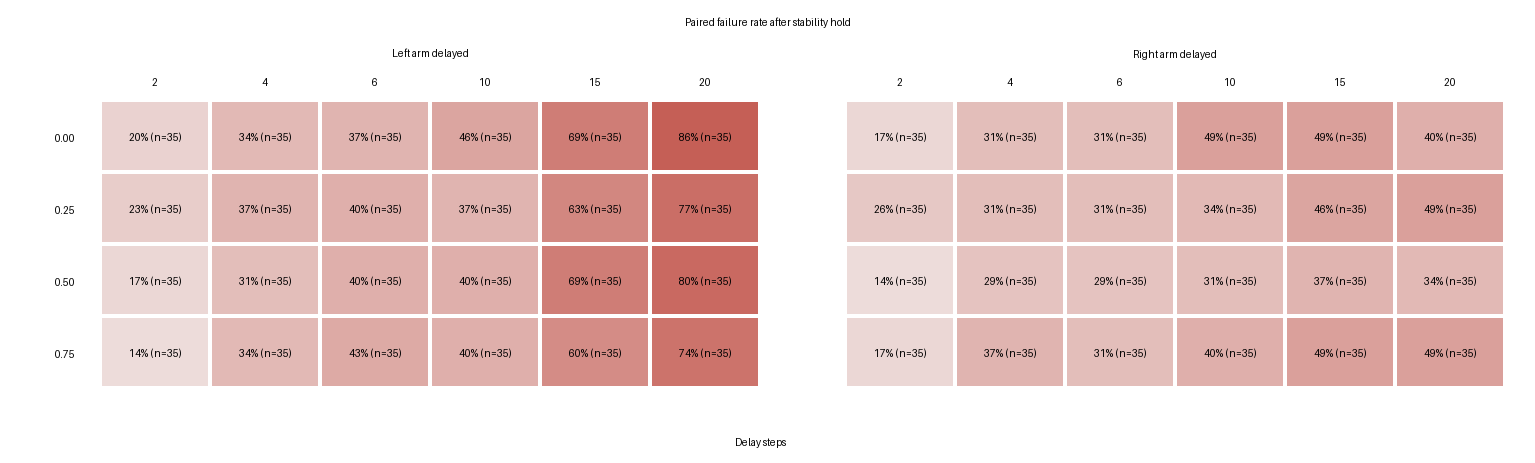
\includegraphics[width=\linewidth]{figures/sensitivity_heatmap.png}
}{
    \begin{tikzpicture}[x=1.05cm,y=0.62cm,font=\small]
        \draw[->] (0,0) -- (6.6,0) node[right]{延迟步数};
        \draw[->] (0,0) -- (0,5.7) node[above]{阶段};
        \foreach \x/\lab in {1/2,2/4,3/6,4/10,5/15,6/20}
            \node[below] at (\x,0) {\lab};
        \foreach \y/\lab in {1/0\%,2/25\%,3/50\%,4/75\%}
            \node[left] at (0,\y) {\lab};
        \foreach \x in {1,...,6}
            \foreach \y in {1,...,4}
                \draw[fill=gray!15] (\x-0.38,\y-0.32) rectangle (\x+0.38,\y+0.32);
        \node[align=center] at (3.5,5.1) {等待完整筛选结果；\\左右臂分别绘图};
    \end{tikzpicture}
}
\caption{协同敏感性热图。颜色表示稳定基线子集上的配对失败率，格内同时标注有效样本数。}
\label{fig:sensitivity_heatmap}
\end{figure}

\subsection{消融实验}

\begin{enumerate}
    \item 去除稳定保持检查，只使用轨迹中任意时刻成功；
    \item 用冻结窗口代替动作完整的后缀延迟，检验动作删除造成的混杂；
    \item 去除困难失败样本或去除协同判别损失；
    \item 不按敏感性筛选，随机选择等量反事实；
    \item 改变延迟集合、阶段数量、保持步数和每条源示范的样本预算；
    \item 在 BC-RNN、ACT 和 Diffusion Policy 上替换基础策略，检验方法的模型无关性。
\end{enumerate}

\subsection{统计检验}

策略评估使用固定测试初始状态并进行配对比较。成功率报告 bootstrap 95\% 置信区间；同一初始状态下的二元成功结果使用 McNemar 检验；多随机种子结果同时报告均值和标准差。涉及多个干预条件时使用 Benjamini--Hochberg 方法控制错误发现率。默认显著性水平设为 $0.05$，bootstrap 重采样10000次。除显著性外同时报告绝对成功率差和置信区间，避免只依赖 $p$ 值。

\subsection{失败模式分析}

除成功率外，随机抽取并人工复核失败轨迹，将其归入以下类别：未建立关键接触、接触建立过早或过晚、支撑手失稳、物体滑移、发生非目标碰撞、到达任务区域但保持后退出。对每类至少展示一个基线—反事实配对案例，并报告不同方法的失败构成。该分析用于回答性能变化是否确实来自协同时序，而不是控制器数值不稳定或仿真异常。

\section{结论与局限}

本文研究少量双臂示范下的协同时序数据生成问题，并提出\method{}。该方法通过动作完整的单臂后缀延迟构造受控反事实，在物理仿真中识别双臂协同敏感阶段，再将成功近邻和困难失败样本用于策略学习。其核心出发点是：运动学上可达并不保证物理上可执行，而相对时序是接触丰富双臂任务中不可忽略的变量。

当前方案仍有四点局限。第一，插入等待虽然保留了动作序列，但系统状态在等待期间发生变化，因此它是面向执行因果性的干预，而不是严格保持所有其他变量不变的统计反事实。第二，delta 动作完整并不等价于末端状态完全一致，控制器闭环误差和接触动力学仍会改变最终状态。第三，仿真接触模型和真实机器人之间存在差距，仿真中得到的敏感边界需要少量实机试验校准。第四，单一任务上的非单调响应可能来自特定接触几何，必须通过更多任务和初始条件验证其普遍性。

后续工作将研究从第一视角人类视频或跨具身重定向轨迹中恢复阶段语义，并用语义阶段约束替代固定比例窗口；同时探索使用视觉语言模型辅助识别“支撑、对齐、插入、释放”等协同阶段。\todo{根据最终实验结果重写本节，避免重复摘要。}


\bibliographystyle{unsrtnat}
\bibliography{references}

\appendix
\section{实现与复现细节}
\label{app:implementation}
\begin{itemize}
    \item 数据集：DexMimicGen TwoArmThreading，1025 条示范，共 218858 个时间步。
    \item 控制频率：20 Hz；动作维度：右臂 7 维加左臂 7 维。
    \item 稳定成功：轨迹结束后继续保持末端动作 $H$ 步，最后一帧仍满足任务成功条件。
    \item 代码入口：\texttt{coordination\_pipeline.py}；统计入口：\texttt{analyze\_coordination\_results.py}。
    \item \todo{补充随机种子、GPU、训练轮数、网络结构和超参数。}
\end{itemize}

\section{软件流程验证}
\label{app:pipeline}

为区分“研究结论”与“软件链路可运行”，表~\ref{tab:pipeline_check}记录投稿实验之前的工程验证。这里的数值只用于发现数据格式和训练接口错误，不参与方法有效性的论证。

\begin{table}[h]
\centering
\caption{端到端软件流程验证。}
\label{tab:pipeline_check}
\begin{tabular}{lll}
\toprule
环节 & 验证内容 & 当前状态 \\
\midrule
完整数据 & 1025条轨迹、218858步、哈希与HDF5深检 & 通过 \\
反事实执行 & 基线、逐臂后缀延迟、稳定保持与断点续跑 & 通过 \\
结果分析 & 配对统计、Wilson置信区间、热图与LaTeX表格 & 通过 \\
训练集导出 & states/actions/obs/next\_obs及干预元数据 & 通过 \\
训练接口 & robomimic读取396步冒烟数据并完成2轮BC & 通过 \\
策略效果 & 多数据规模、多随机种子和闭环成功率 & \todo{待完成} \\
\bottomrule
\end{tabular}
\end{table}

\end{document}
